\subsection{Related work}

\begin{itemize}

	\item Moreno made a proposition of IaaS architecture \cite{moreno2012iaas}.	
	
	\item He identified a list of services that are vital for building IaaS that will be usable in production condition for commercial company.

	\item We aim at making a research prototype: we want to keep what is vital for running virtual machines.

\end{itemize}

\subsection{First iteration on Discovery}

\begin{itemize}

	\item For our first iteration, we keep 4 main services:
		\begin{description}

			\item [Compute manager] : responsible for virtual machines lifecycle.

			\item [Network manager] : responsible for virtual networks.

			\item [Storage manager] : responsible for images and persistent block storage.

			\item [Administrative manager] : responsible for infrastructure management and user permissions.  

		\end{description}


	\item In figure \ref{fig:mcd} we propose a conceptual data model to explain our proposal.


	\begin{figure*}
		\centering
		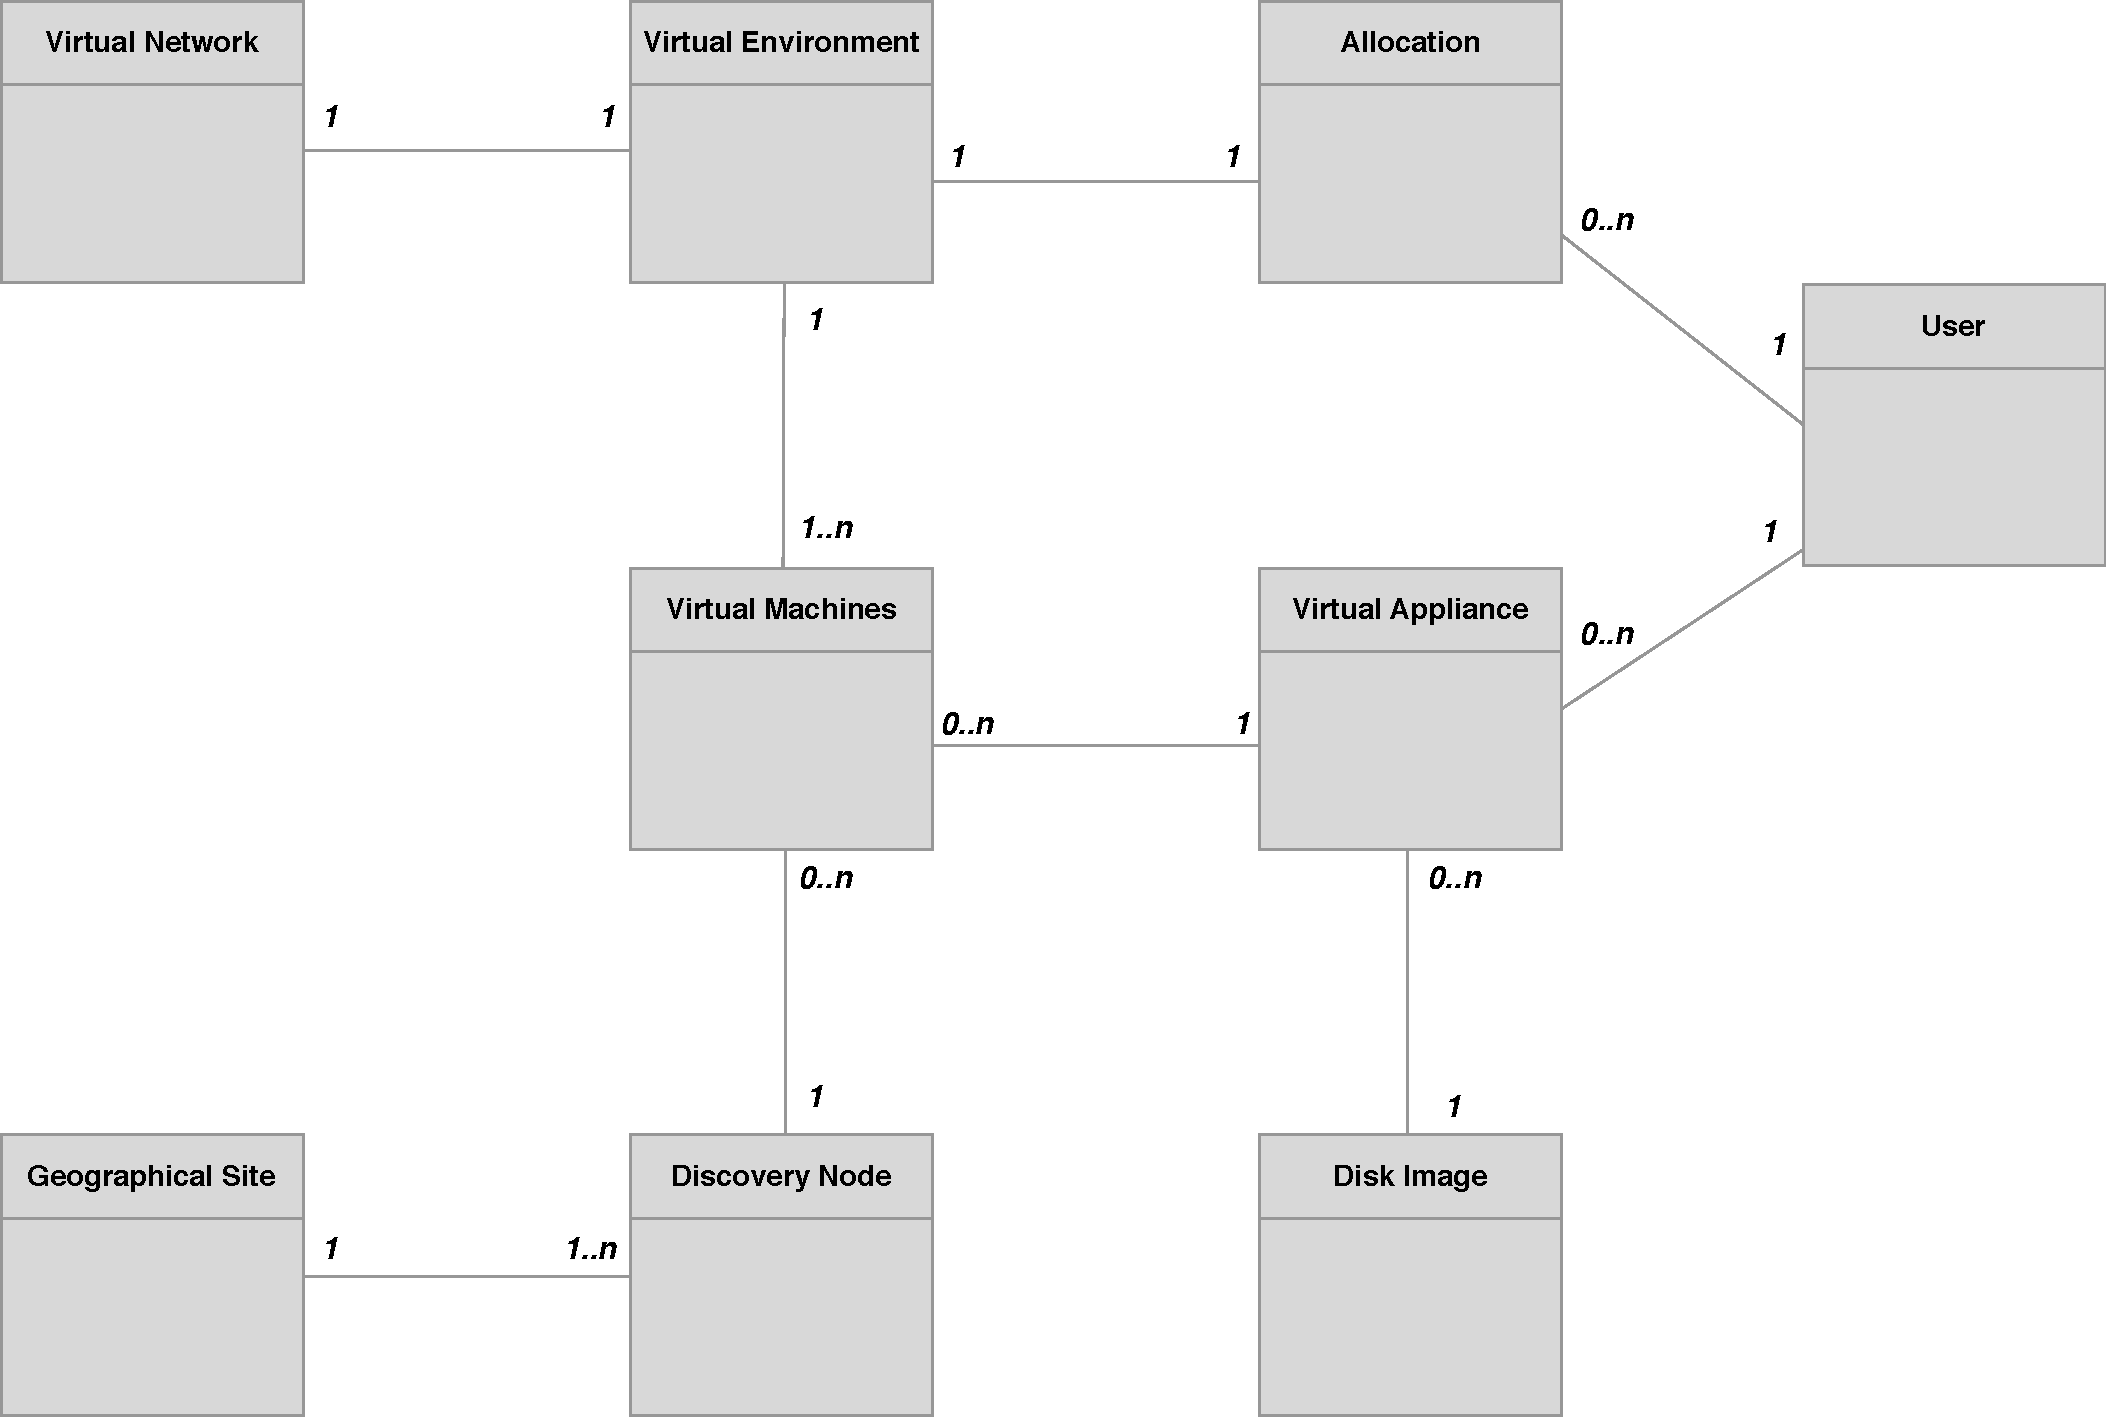
\includegraphics[width=0.75\linewidth]{Figures/mcd_2.pdf}
		\caption{Conceptual Data Model for Discovery proposal.}%
		\label{fig:mcd}%
		%\vspace*{-.8cm}
	\end{figure*}


\end{itemize}